% !TeX root=main.tex

\chapter{مفاهیم پایه} \label{ch:basics}
\thispagestyle{empty}


\section{مقدمه}
\paragraph{}
{
    در این بخش به معرفی مفاهیم پایه از یادگیری عمیق و برخی معماری‌هایی که 
    در این پژوهش استفاده شده‌اند به مانند شبکه‌های عصبی بازگشتی، مکانیزم‌ توجه و معماری
    ترنسفورمرز و مدل‌های کدکذار و کدگشا پرداخته‌شده است.
}


\section{شبکه‌های عصبی مصنوعی}
\label{sec:ann}
\paragraph{}
{
    شبکه‌های عصبی مصنوعی سیستم‌ها و روش‌های محاسباتی نوینی هستند که 
    از گروهی راس‌ به نام نورون‌ها تشکیل شده‌اند که توسط وزن‌هایی به
    یکدیگر متصلند. یک شبکه عصبی از یک لایه ورودی، چندین لایه مخفی و یک لایه
    خروجی تشکیل شده‌است. اگر از دید ریاضیات این شبکه‌ها را بررسی کنیم، می‌توانیم 
    دو لایه را از طریق ماتریس وزن‌ها به یکدیگر متصل کنیم. هر لایه از شبکه‌های عصبی 
    تبدیل به‌خصوصی را به ورودی‌های خود اعمال می‌کنند. در نهایت خروجی‌های هر لایه 
    مطابق با معادله
    \ref{eq:1}
    محاسبه می‌شوند و به لایه‌های بعدی منتقل می‌شوند. 
    \begin{center}
        \begin{equation} \label{eq:1}
            LayerOutput = A(XW + B)
        \end{equation}
    \end{center}

    به هر شبکه مصنوعی یک تابع هزینه نسبت داده‌ شده است که برای کاهش آن
    از مکانیزم‌های بهینه‌سازی استفاده‌ می‌شود. این مکانیزم‌ها برای توابع
    مشتق‌پذیر برپایه گرادیان کاهشی و برای توابع مشتق‌ناپذیر برپایه الگوریتم‌های 
    ژنتیک بنا شده‌اند. بر اساس قضیه تقریب، هر تابع پیوسته را در فضای 
    $\mathbb{R}^n$
    را می‌توان با یک لایه مخفی و یک تابع فعال‌ساز تقریب زد. این قضیه را می‌توان نقطه 
    قوت شبکه‌های عصبی مصنوعی دانست. دلایل اصلی پیشرفت‌های اخیر شبکه‌های عصبی می‌توان
    وجود داده در دسترس، توانایی آموزش مدل‌ها از طریق پردازنده‌های گرافیکی 
    و وجود کتاب‌خانه‌های مشتق‌گیر نظیر 
    \cite{tensorflow2015-whitepaper}
    \lr{Tensorflow}
    و 
    \cite{NEURIPS2019_9015}
    \lr{Pytorch}
    نام برد. 
}

\section{شبکه‌های عصبی بازگشتی}
\label{sec:rnn}
\paragraph{}
{
    باید توجه داشت که استفاده از شبکه‌های عصبی مصنوعی برای داده‌های دنباله‌ای عملی
    نیست. به عبارتی دیگر در شبکه‌های عصبی مصنوعی فرض می‌کنیم که داده‌های ورودی به صورت
    کامل مستقل از یکدیگرند. با توجه به این فرضیه شبکه‌های عصبی مصنوعی عادی برای 
    استخراج وابستگی بین دنباله‌ها 
    (برای مثال کلمات درون یک جمله)
    کارآمد نیستند. برای در نظر گرفتن این وابستگی، از شبکه‌های عصبی بازگشتی استفاده
    می‌شود. 

    شبکه‌های عصبی بازگشتی را می‌توان همان شبکه‌های عصبی عادی با یک حافظه در نظر گرفت.
    در واقع مهم‌ترین تفاوت شبکه‌های عصبی بازگشتی وجود حالت‌های مخفی است که می‌توانند 
    اطلاعات گذشته را در حافظه نگه دارند و سپس از طریق پس‌انتشار خطا در راستای زمان 
    به کاهش تابع هزینه کمک کنند. قابلیت به یاد سپردن گذشته شبکه‌های عصبی بازگشتی را
    بسیار کارآمد کرده است. در واقع شبکه‌های عصبی بازگشتی با تعداد پارامترهای محدود
    تورینگ‌‌کامل هستند و توانایی پیاده‌سازی هر الگوریتمی را دارند. 
    \cite{sontag1995computational}

    \begin{figure}[H]
     \center{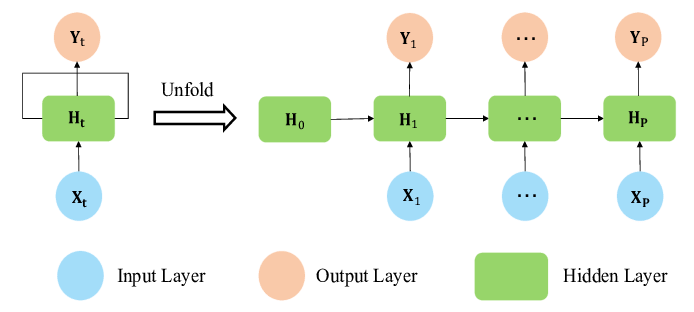
\includegraphics[width=0.7\textwidth]{figs/RNN_ARC_1.png}}
     \caption{معماری کلی شبکه‌های عصبی بازگشتی}
     \label{fig:rnn_1}
    \end{figure}

    یکی از مشکلات متداول شبکه‌های عصبی بازگشتی، محو شدگی و انفجار گرادیان
    به صورت نمایی در گذر زمان است. این مسئله بدان معنی است که این معماری‌ها 
    توانایی پردازش دنباله‌هایی با وابستگی‌های طولانی را ندارند. برای حل این‌ مشکل
    معماری‌های متفاوتی ارائه شد که به بررسی مهم‌ترین آن‌ها می‌پردازیم. 
}

\subsection{
    حافظه طولانی کوتا‌ه‌مدت
}
\label{subsec:lstm}
\paragraph{}
{
    در سال 1977 یک معماری از شبگه‌های عصبی بازگشتی به نام  حافظه طولانی کوتا‌ه‌مدت 
    ارائه شد. هر عنصر از شبکه شامل یک درگاه ورودی، یک سلول، یک درگاه
    فراموشی و یک درگاه خروجی است. سلول طولانی کوتا‌ه‌مدت وظیفه یادآوری 
    مقادیر دیده‌شده در گذشته را برعهده دارد، در حالی که درگاه‌های ورودی، 
    فراموشی و خروجی وظیفه کنترل جریان داده‌ها را دارند. 

    \begin{figure}[H]
        \center{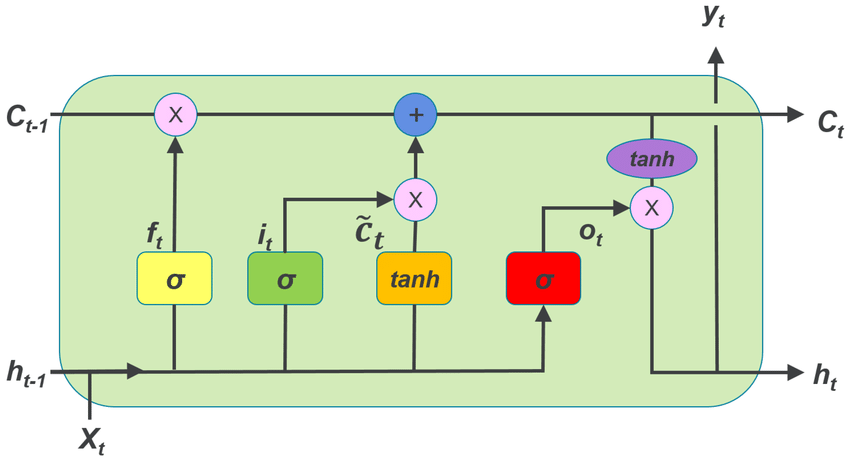
\includegraphics[width=0.7\textwidth]{figs/LSTM_ARC_1.png}}
        \caption{معماری حافظه کوتاه‌مدت طولانی‌مدت}
        \label{fig:lstm_1}
    \end{figure}
   
    از آنجایی که هدف اصلی حل محوشدگی نمایی گرادیان در طول زمان بود، حافظه‌های 
    طولانی کوتا‌ه‌مدت قابلیت پردازش دنباله‌های طولانی‌‌تری را دارند. معادلات مرتبط با
    این شبکه‌ها در زیر آورده شده است.

    \begin{center}
        \begin{equation} \label{eq:2}
            \sigma (x) = \frac{1}{1 + e ^{-x}}
        \end{equation}
        \begin{equation} \label{eq:3}
            tanh(x) = \frac{e^{2x} - 1}{e^{2x} + 1}
        \end{equation}
        \begin{equation} \label{eq:4}
            i_t = \sigma (W_i^T x_t + W_i^T h_{t - 1} + b_i)
        \end{equation}
        \begin{equation} \label{eq:5}
            f_t = \sigma (W_f^T x_t + W_f^T h_{t - 1} + b_f)
        \end{equation}
        \begin{equation} \label{eq:6}
            o_t = \sigma (W_o^T x_t + W_o^T h_{t - 1} + b_o)
        \end{equation}
        \begin{equation} \label{eq:7}
            c_t = f_t \circ c_{t - 1} +
                i_t \circ tanh(W_c x_t + U_c h_{t - 1} + b_c)
        \end{equation}
        \begin{equation} \label{eq:8}
            h_t = o_t \circ tanh(c_t)
        \end{equation}
    \end{center}

    سلول 
    (معادله \ref{eq:8})
    وابستگی‌های بین مقادیر ورودی در دنباله را نگه می‌دارد. درگاه ورودی
    (معادله \ref{eq:4})
    وظیفه انتخاب ویژگی‌های ورودی برای عبور به سلول را عهده‌دار است. 
    درگاه فراموشی 
    (معادله \ref{eq:5})
    میزان این که یک مقدار چقدر در سلول باقی بماند را برعهده دارد و در نهایت 
    درگاه خروجی، میزان مشارکت مقادیر موجود در سلول را برای محاسبه خروجی را 
    کنترل می‌کند. 
}

\subsection{
    واحد بازگشتی دروازه‌دار    
}
\label{subsec:rep_learn}
\paragraph{}
{
   در سال 2014 شبکه‌های واحد بازگشتی دروازه‌دار به عنوان معماری متفاوتی برای
   شبکه‌های عصبی بازگشتی ارائه شد تا مشکل محوشدگی گرادیان‌ در حال آموزش را حل کند.
   این واحد شباهت زیادی به حافظه طولانی کوتاه‌مدت دارد ولی در عین‌ حال تعداد
   پارامترهای کمتری دارد و در نتیجه سریع‌تر آموزش می‌بیند. 

   \begin{center}
        \begin{equation} \label{eq:9}
            z_t = \sigma (W_z x_t + U_z h_{t - 1} + b_z)
        \end{equation}
        \begin{equation} \label{eq:10}
            r_t = \sigma (W_r x_t + U_r h_{t - 1} + b_r)
        \end{equation}
        \begin{equation} \label{eq:11}
            \hat{h_t} = tanh (W_h x_t + U_r (r_t \circ h_{t - 1}) + b_h)
        \end{equation}
        \begin{equation} \label{eq:12}
            h_t = (1 - z_t) \circ h_{t - 1} + z_t \circ \hat{h_t}
        \end{equation}
    \end{center}
    
    مطابق با معادله 
    \ref{eq:9}
    درگاه $z_t$
    مسئولیت تعیین عبور مقادیر برای استفاده در آینده را دارد. به عبارتی اگر 
    مقدار آن برابر 1 باشد، بدان معنی است که شبکه مقدار بردار 
    $h_t$ 
    را به صورت کامل به‌روز و اطلاعات گذشته را فراموش می‌کند. متقابلا اگر 
    مقدار این درگاه به 0 نزدیک باشد، شبکه مقادیر $h_t$ 
    را از گذشته انتخاب می‌کند. درگاه فراموشی، مطابق با معادله
    \ref{eq:10}
    مسئولیت تعیین تاثیرگذاری مقادیر حالت قبلی در محاسبه حالت فعلی را بر عهده‌دارد.

    \begin{figure}[H]
        \center{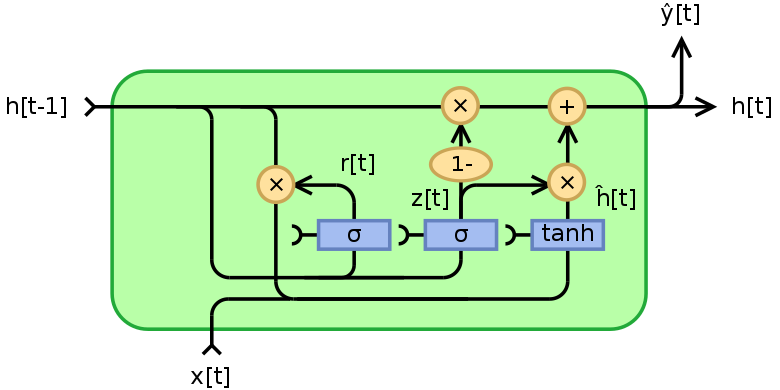
\includegraphics[width=0.7\textwidth]{figs/GRU_ARC_1.png}}
        \caption{معماری شبکه واحد بازگشتی دروازه‌دار}
        \label{fig:gru_1}
    \end{figure}
}
\section{مدل‌های دنباله‌به‌دنباله}
\label{sec:seq2seq}
\paragraph{}{
    مدل‌های دنباله‌به‌دنباله وظیفه تبدیل دنباله‌ها از یک دامنه به دنباله‌ای دیگر 
    را برعهده دارند. به طور کلی این مدل‌ها دنباله‌ای با طول متغیر را ورودی می‌گیرند و
    دنباله‌ای دیگر با طول متغیر بدل می‌کنند کع لزما طول آن با ورودی یکسان نیست. 
    مدل‌های دنباله‌به‌دنباله دارای دو شبکه مجزا هستند. یک شبکه به عنوان کدگذار
    که وظیفه تبدیل ورودی‌ها به یک یا چند بردار ویژگی را برعهده دارد. 
    این بردار ویژگی یک بازنمایی از دنباله ورودی است که حداکثر معانی قابل
    استخراج از دنباله ورودی را در بر دارد. شبکه دیگری با عنوان کدگشا 
    برای تولید دنباله هدف آموزش می‌بیند. ورودی این بخش همان بردار ویژگی 
    بدست آمده از کدگذار است. معمولا شبکه‌های کدگذار و کدگشا با یکدیگر آموزش
    داده می‌شوند که به معنی پس انتشار خطا از کدگشا به کدگذار است. در شکل
    \ref{fig:enc_dec_1}
    نمونه‌ای از مدل‌های دنباله‌به‌دنباله را برای حل ترجمه ماشینی مشاهده می‌شود. 
    \begin{figure}[H]
        \center{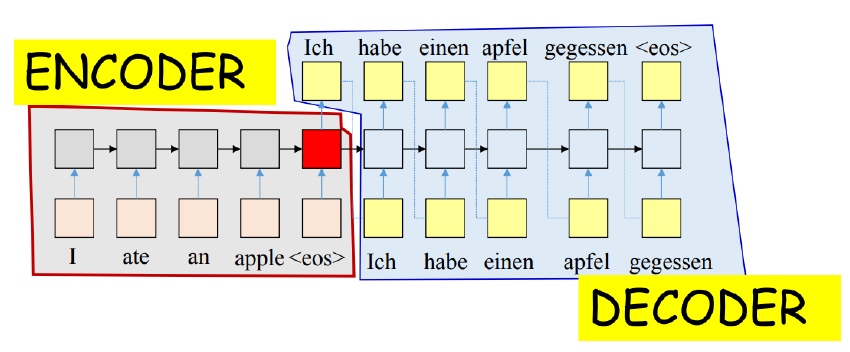
\includegraphics[width=0.7\textwidth]{figs/enc_dec.png}}
        \caption{نمونه‌ای از معماری‌ کدگذار-کدگشا برای حل مسئله ترجمه ماشینی}
        \label{fig:enc_dec_1}
    \end{figure}
}
\section{مکانیزم توجه}
\label{sec:attn}
\paragraph{}{
    شبکه‌های عصبی بازگشتی و معماری‌های مشابه آن می‌توانند اطلاعات درون یک 
    دنباله را پردازش کنند و بر اساس آن‌ها نتیجه گیری کنند. حال فرض کنیم
    که یک پاراگراف طولانی داریم و پس از خواندن آن سوالی پرسیده شود.
    پس از روبه‌رو شدن با سوال، ممکن است متن را به صورت کامل به یاد نیاوریم
    و لازم باشد که دوباره با توجه بیشتری به برخی جملات متن را بخوانیم.
    بنابراین، توجه را می‌توانیم رفتار تمرکز بر روی بخش گسسته‌ای از اطلاعات 
    و در نظر نگرفتن دیگر اجزاء تعریف کنیم. در ادامه به ایده‌ها و انواع 
    مکانیزم‌های توجه ارائه شده در طی سال‌های گذشته می‌پردازیم.
}
\subsection{
    مکانیزم توجه باهدانا 
    (\lr{Bahdanau})
}
\label{subsec:bahdanau_attn}
\paragraph{}{
    در سال 2014 مکانیزمی 
    \cite{DBLP:journals/corr/BahdanauCB14}
    برای توجه به حالت‌های مخفی در محاسبه خروجی ارائه داد. در این معماری 
    علاوه بر حالت سلول کدگذار آخر، تمام خروجی‌های کدگذار را به کدگشا می‌فرستیم
    تا در هر گام، کدگشا یک جمع وزن‌دار بین خروجی‌ها حساب کند. وزن‌های این جمع، 
    مفهوم توجه را پیاده‌سازی می‌کنند. هر حالتی که وزن بیشتری داشته‌باشد توجه
    بیشتری را جلب می‌کند‍!
    \begin{figure}[H]
        \center{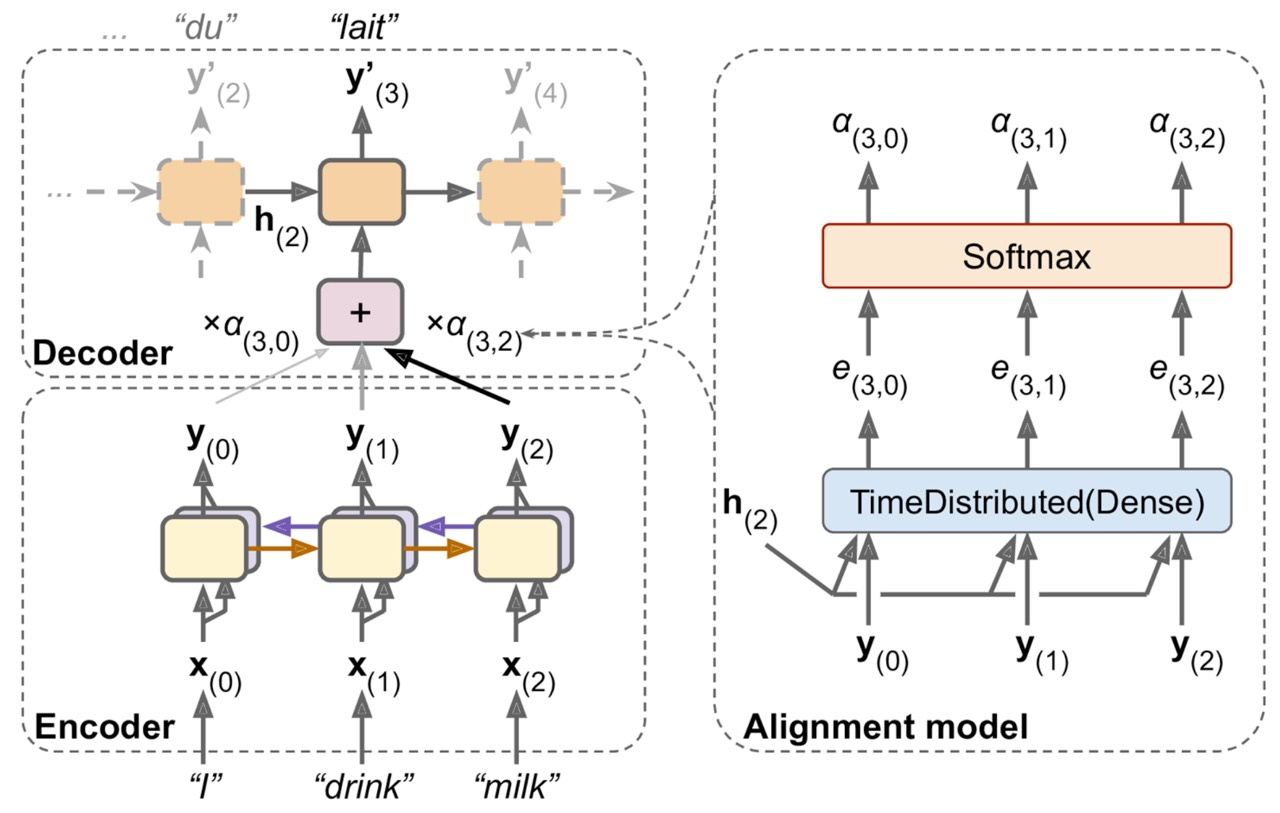
\includegraphics[width=0.7\textwidth]{figs/bahdanau_attn_1.jpeg}}
        \caption{مکانیزم توجه باهدانا در ترجمه ماشینی}
        \label{fig:bahdanau_attn}
    \end{figure}

    وزن‌های مذکور همان 
    $\alpha$
    موجود در شکل
    \ref{fig:bahdanau_attn}
    که همراه با شبکه آموزش می‌بینند. با توجه به شکل متوجه می‌شویم به هنگام
    ترجمه کلمه 
    \lr{lait}
    ،
    توجه بیشتری به کلمه متناظر آن که 
    \lr{milk}
    است، می‌شود. در ادامه به بررسی فرمول‌های مکانیزم توجه باهدانا می‌پردازیم. 

    \begin{center}
        \begin{equation} \label{eq:13}
            e_{t, i} = a(s_{t - 1}, h_i)
        \end{equation}
        \begin{equation} \label{eq:14}
            a(s_{t - 1}, h_i) = v^T tanh( W[{h_i; s_{t - 1}}] )
        \end{equation}
        \begin{equation} \label{eq:15}
            a(s_{t - 1}, h_i) = v^T tanh( W[{W_1 h_i + W_2 s_{t - 1}}] )
        \end{equation}
        \begin{equation} \label{eq:16}
            \alpha_{t, i} = softmax(e_{t, i})
        \end{equation}
    \end{center}

    با توجه به معادله 
    \ref{eq:16}،
    برای محاسبه مقادیر 
    $\alpha$
    لازم است از تابع تناظر 
    $a$ 
    استفاده کنیم که برای محاسبه آن نیز دو روش الحاق 
    (معادله \ref{eq:14})
    و جمع 
    (معادله \ref{eq:15})
    وجود دارد. 
    در نهایت با استفاده از یک لایه 
    softmax
    به محاسبه وزن‌ها می‌پردازیم. 
}

\subsection{
    مکانیزم توجه لوآنگ 
    (\lr{Luong})
}
\label{subsec:loung}
\paragraph{}{
    در سال 2015،
    مقاله‌ای دیگر 
    \cite{luong-etal-2015-effective}
    مدل مکانیزم دیگری ارائه داد. از آنجایی که هدف مکانیزم توجه، 
    محاسبه شباهت‌های بین خروجی‌های کدگذار و حالت‌های پنهان مراحل قبل کدگشا است،
    در این مقاله نیز از ضرب کسینوسی استفاده شده است. همانطوری که از معادلات
    زیر مشخص است، توجه لوآنگ، بر خلاف توجه باهدانا، از حالت پنهان 
    $s_t$
    استفاده می‌کند. 

    \begin{center}
        \begin{equation} \label{eq:17}
            a(s_{t}, h_i) = v_a^T tanh( W[{h_i; s_{t}}] )
        \end{equation}
        \begin{equation} \label{eq:18}
            a(s_{t}, h_i) = s_t^T h_i
        \end{equation}
        \begin{equation} \label{eq:19}
            a(s_{t}, h_i) = s_t^T W_a h_i
        \end{equation}
    \end{center}
}

\subsection{
    مکانیزم توجه به خود
}
\label{subsec:self_attn}
\paragraph{}{
    این مفهوم برای اولین بار در سال 2016 مطرح شد.
    \cite{cheng-etal-2016-long}
    هدف این توجه
    این‌است که ارتباط اجزای موجود در یک دنباله را با یکدیگر بسنجد
    تا بتواند برداشت درست‌تری از کل دنباله داشته باشد. تنها تفاوت 
    این مکانیزم با توجه عادی این است میزان توجه اجزا دنباله را با خود
    همان دنباله می‌سنجیم. شکل
    \ref{fig:self_attention}
    ارتباط کلمه‌ قرمز رنگ با کلمه‌های قبلی در جمله بررسی شده و شدت آبی بودن
    هر کلمه، میزان ارتباط را نشان می‌دهد. 
    \begin{figure}[H]
        \center{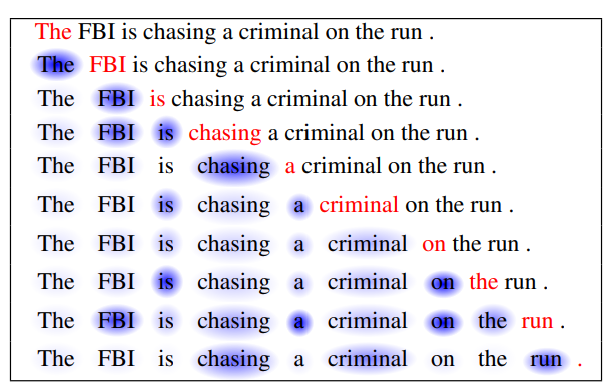
\includegraphics[width=0.7\textwidth]{figs/self_attn_1.png}}
        \caption{نمونه‌ای از توجه به خود در یک جمله}
        \label{fig:self_attn_1}
    \end{figure}
}


\section{
    مدل‌های transformer و مکانیزم توجه آن‌ها
}
\label{sec:transformers}
\paragraph{}{
    مدل‌های تبدیل‌کننده روش جدیدی را برای استفاده‌ از مفهوم توجه ارائه دادند.
    در مقاله‌‌ی «توجه و دیگر هیچ!» 
    \cite{NIPS2017_3f5ee243}
    که در سال 2017 ارائه شد، این مدل‌ها مطلقا بر پایه 
    مکانیزم توجه به خود تکیه کرده‌اند. اکثر این مدل‌ها به صورت 
    مدل‌های دنباله‌به‌دنباله پیاده‌سازی شده‌اند به صورتی که دو بخش
    کدگذار و کدگشا دارند. مطابق با شکل
    \ref{fig:transformers_arc_1}
    مشاهده‌ می‌کنیم که بخشی به نام  
    \lr{Positional Embedding}
    شرایط پردازش کلمات با توجه به جایگاه آن‌ها در جمله را فراهم می‌کند. 
    برای این کار از معادلات 
    \ref{eq:20} و \ref{eq:21}
    بردارهای جایگاه محاسبه می‌شوند و به بردار‌های 
    \lr{embedding}
    اضافه می‌شوند. 
    \begin{center}
        \begin{equation} \label{eq:20}
            PE(pos, 2i) = sin(\frac{pos}{10000^{\frac{2i}{d}}})
        \end{equation}
        \begin{equation} \label{eq:21}
            PE(pos, 2i + 1) = cos(\frac{pos}{10000^{\frac{2i}{d}}})
        \end{equation}
    \end{center}
    \begin{figure}[H]
        \center{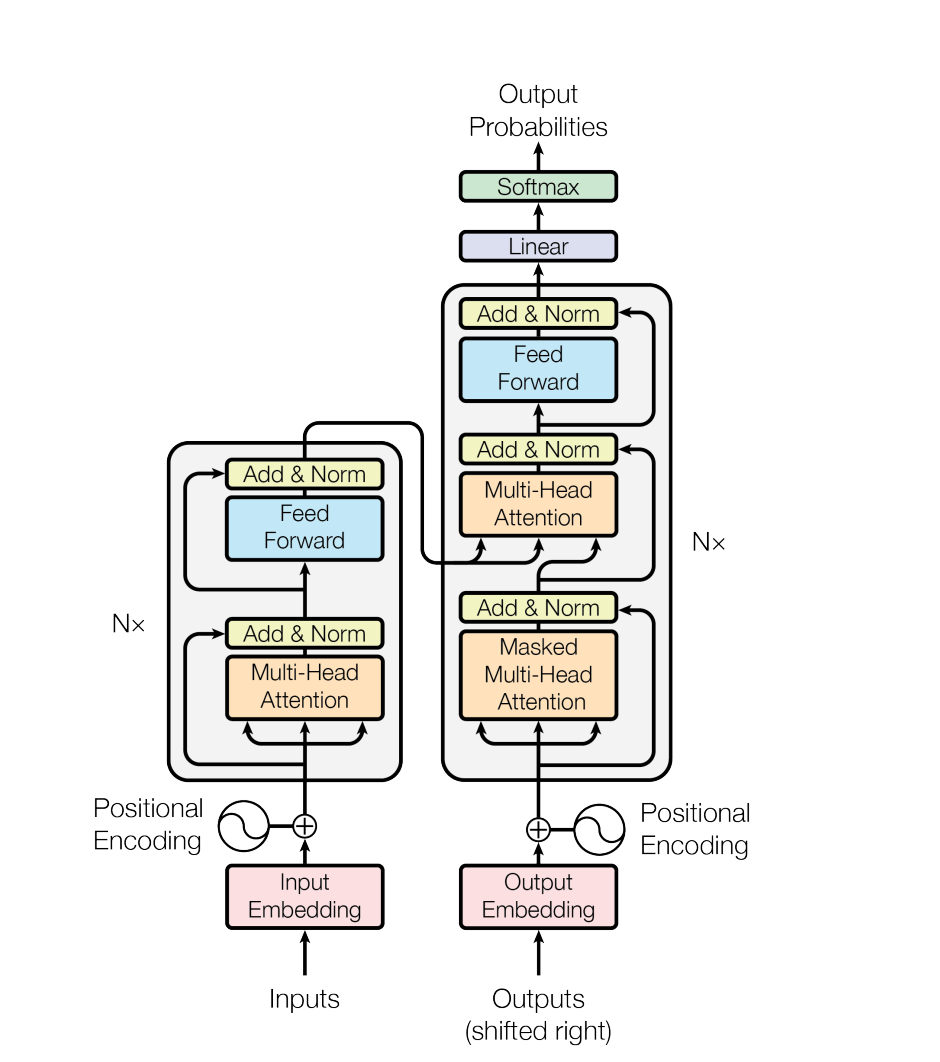
\includegraphics[width=0.7\textwidth]{figs/transformers_arc_1.png}}
        \caption{مدل‌ تبدیل‌شونده و معماری آن‌}
        \label{fig:transformers_arc_1}
    \end{figure}

    همان‌طوری که در شگل 
    \ref{fig:transformers_arc_1} 
    مشخص است، شبکه‌های کدگذار و کدگشا از توجه چندسر استفاده می‌کنند. 
    این نوع از مکانیزم توجه را می‌توان تعمیم‌یافته‌ی نسخه قبلی آن دانست. 
    در توجه چندسر ما با سه موجودیت مختلف به نام کلید 
    (\lr{Key})، 
    مقدار 
    (\lr{Value})
     و پرسش 
    (\lr{Query})
    سروکار داریم. 
    در مبحث توجه گفتیم که هدف این کار، تعیین میزان ارتباط بین هر جزء جمله خروجی
    با تمامی اعضای جمله ورودی است.
    اگر به شکل 
    \ref{fig:transformers_arc_1} 
    توجه کنید، می‌بینید که هر سه ورودی این بلوک توجه 
    از یک منبع که همان جمله‌ی ورودی است می‌آیند، پس از نوع توجه به خود  
    است و هدف آن تعیین ارتباط و درک بهتر اجزای جمله‌ی زبان مبدا به یکدیگر است.
    پیش از بررسی ادامه‌ی روند مدل، لازم است تا الگوریتمی
    که در این نوع از مکانیزم توجه دنبال می‌شود را بررسی کنیم.
    
    \begin{figure}[H]
        \center{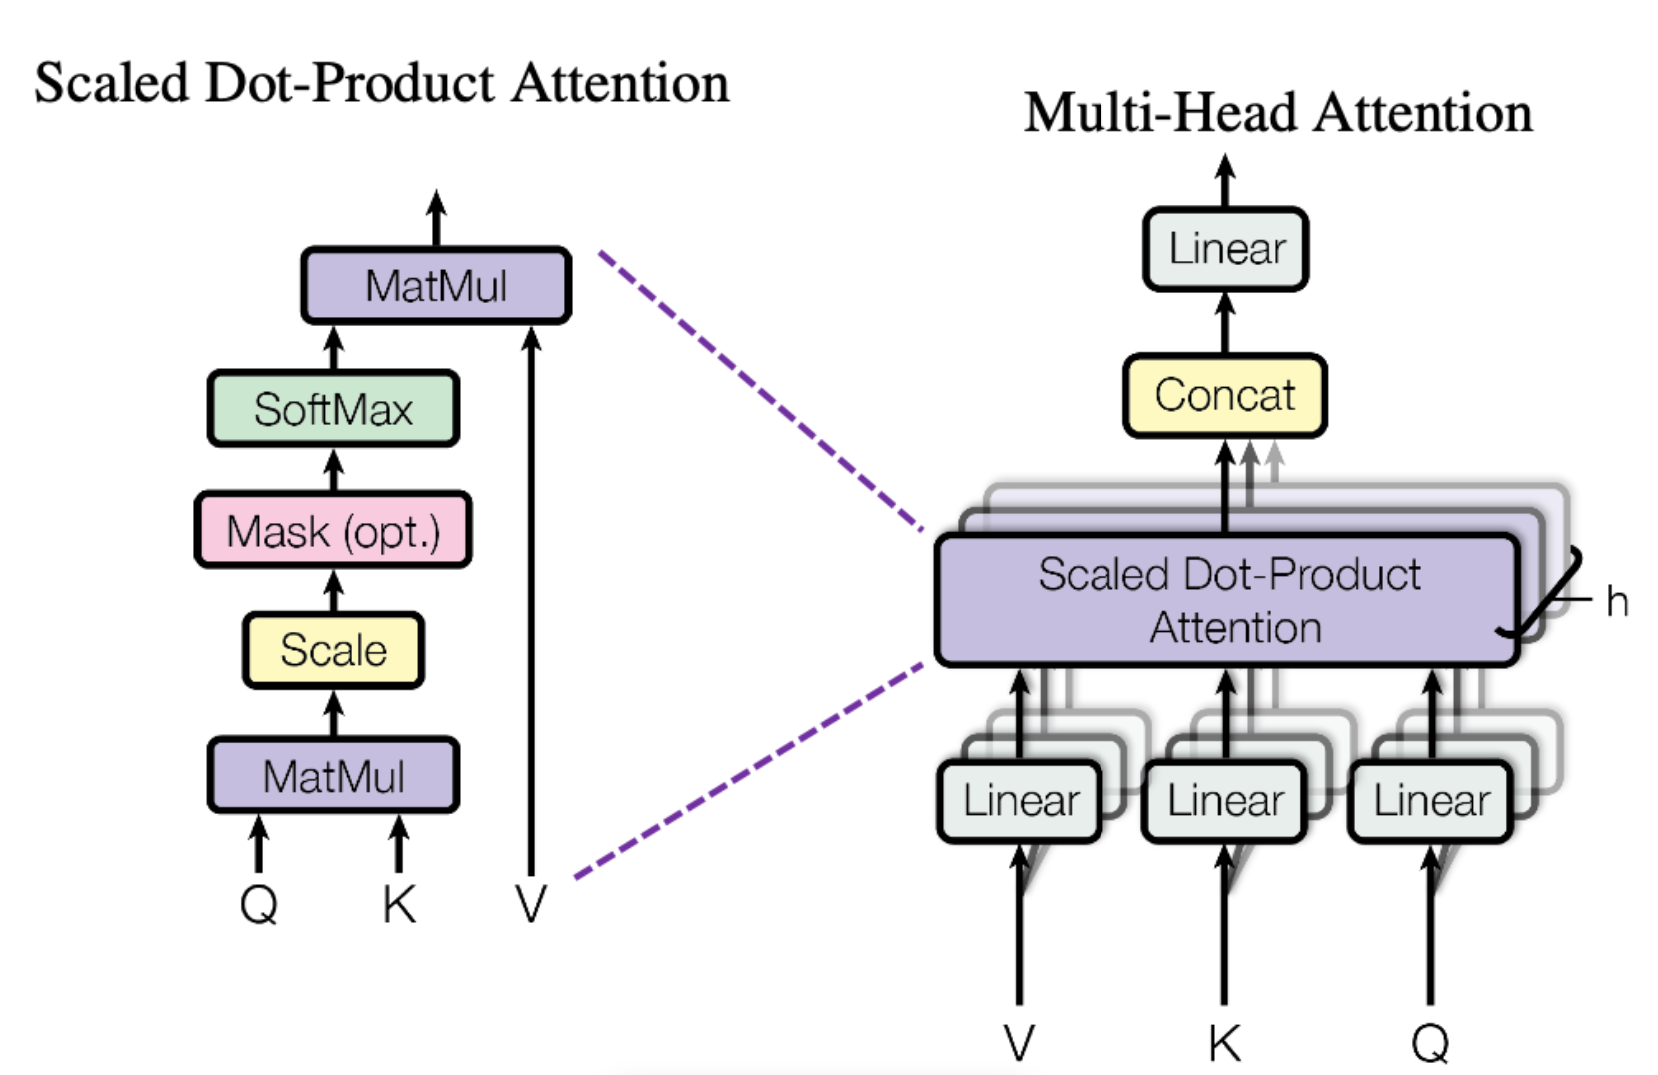
\includegraphics[width=0.7\textwidth]{figs/multihead_attn_1.png}}
        \caption{توجه چندسر و توجه مقیاس‌شده بر پایه ضرب داخلی}
        \label{fig:multihead_attn_1}
    \end{figure}

    در مرحله‌ی اول، بردار کلمات با گذر از سه لایه‌ی پیش‌خور 
    (\lr{feed-forward layer})
    با وزن‌های متفاوت، وکتورهای 
    \lr{K}، \lr{V} و \lr{Q} 
    را می‌سازند. سپس این وکتورها، وارد بلوک توجه مقیاس‌شده‌ی بر پایه‌ی ضرب داخلی
    (\lr{Scaled Dot-Product Attention})
    می‌شوند. در این بخش، ابتدا ضرب داخلی وکتورهای 
    \lr{Q} و \lr{K} 
    محاسبه می‌شود تا مشخص شود این دو چقدر به هم شبیهند.
    سپس، با تقسیم امتیاز حاصل بر جذر طول رشته‌ی ورودی، 
    امتیاز نرمال می‌شود تا از بروز مشکل انفجار گرادیان جلوگیری شود.
    سپس، با اعمال تابع 
    \lr{softmax}
    بر روی این مقادیر، وزن هر کدام از کلیدها برای هر پرسش 
    (\lr{query}) 
    تعیین می‌شود. در نهایت، وزن‌های محاسبه‌شده در مقدارهای 
    (\lr{value})
    کلمات متفاوت ضرب می‌شوند تا خروجی مورد نظر تولید شود. 
    این مراحل را می‌توانید در تصویر
    \ref{fig:multihead_attn_1}
    مشاهده کنید.
    با توجه به این که کدگشا رشته‌ی خروجی را کلمه به کلمه تولید می‌کند،
    باید درنظر داشته باشیم که وزن‌های توجه به گونه‌ای نباشند که کلمات به
    واژه‌های بعد از خود توجه داشته باشند.

    برای این کار، در روند توجه مقیاس‌شده‌ی بر پایه‌ی ضرب داخلی 
    (\lr{Scaled Dot-Product Attention})
    ، بعد از نرمال شدن امتیازها و قبل از اعمال تابع 
    \lr{softmax}
    ، آن‌ را با یک ماتریس اکیدا
    بالا مثلثی که مقادیر بالای قطر اصلی آن منفی بی‌نهایت هستند جمع می‌کنیم.
    این کار باعث می‌شود که بعد از اعمال تابع 
    \lr{softmax}
    ، مقدار وزن توجه هر کلمه به کلمه‌های بعد از خودش صفر شود. نمونه‌ای 
    از این عمل سرپوش گذاری را می‌توانید در معادله
    \ref{eq:22}
    مشاهده کنید. 

    \begin{center}
        \begin{equation} \label{eq:22}
           \begin{bmatrix}
                0.7 & 0.1 & 0.1 & 0.1 \\
                0.1 & 0.6 & 0.2 & 0.1 \\
                0.1 & 0.2 & 0.6 & 0.1 \\
                0.1 & 0.3 & 0.3 & 0.3
           \end{bmatrix}
            +
            \begin{bmatrix}
                0 & -inf & -inf & -inf \\
                0 & 0 &  -inf & -inf \\
                0 & 0 &  0 &   -inf\\
                0 & 0 &  0 & 0
           \end{bmatrix} 
           =
           \begin{bmatrix}
            0.7 & -inf & -inf & -inf \\
            0.1 & 0.6 &  -inf & -inf \\
            0.1 & 0.2 &  0.6 &   -inf\\
            0.1 & 0.3 &  0.3 & 0.3
       \end{bmatrix} 
        \end{equation}
    \end{center}
}
\section{
    مدل‌های زبان و تصویر بر پایه 
    \lr{BERT}
}
\label{sec:bertlike_arcs}
\paragraph{}
{
    مدل‌‌های تصویر و زبان خیرا شهرت بسیاری پیدا کرده‌اند. بر اساس وظیفه اعمال شده، 
    معماری‌های متفاوتی برای حل مسائل تصویر و زبان در کنار یکدیگر ارائه شده است.
    ر آنجایی که تبدیل کنندگان در بسیاری از موارد به خوبی عمل کردند، استفاده
    از آن‌ها برای حل این مسائل اجنتاب‌ناپذیر است. بسیاری از این مدل‌های رائه‌شده
    برپایه 
    \lr{BERT}
    یا معماریی مشابه با آن دارند. به طور کلی می‌توان این مدل‌ها را در دو دسته جای داد.
}
\subsection{
    مدل‌های تک‌جریان
}
\label{subsec:single-stream-models}
\paragraph{}
{
    معماری‌هایی هستند که هر دو بخش تصویر و زبان را در یک ماژول کدگذاری می‌شوند. 
    همانطوری که در تصویر 
    \ref{fig:single_stream}
    مشخص است، بردار‌های تصویر و زبان هردو از یک ماژول تبدیل کننده عبور می‌کنند. 
    مدل‌های تک‌جریان از لحاظ تعداد پارامترها بهینه هستند و از ابتدا به صورت 
    تلفیقی بین بردار‌های تعبیه تصاویر و زبانی تناظر ایجاد می‌کنند.
    \begin{figure}[H]
        \center{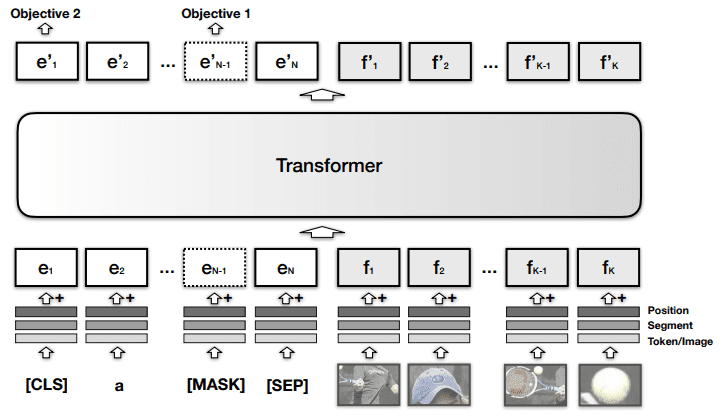
\includegraphics[width=0.6\textwidth]{figs/single_stream_arc.png}}
        \caption{نمونه‌ای از یک مدل تک‌جریان}
        \label{fig:single_stream}
    \end{figure}
}

\subsection{
    مدل‌های دوجریان
}
\label{subsec:dual-stream-models}
\paragraph{}
{
    معماری‌هایی هستند که بخش تصویر و زبان در ماژول‌های جداگانه پردازش می‌شوند و 
    سپس توسط ماژول دیگری ارتباط بین بردار‌های تعبیه شده زبانی با بردارهای 
    تصویر را محاسبه می‌کند. 
    با توجه به تصویر
    \ref{fig:dual_stream}
    هر دو بخش تصویر و زبان جداگانه جریان پیدا می‌کنند و سپس
    یک تناظر بین این دو جریان بدست می‌آوریم. 
    \begin{figure}[H]
        \center{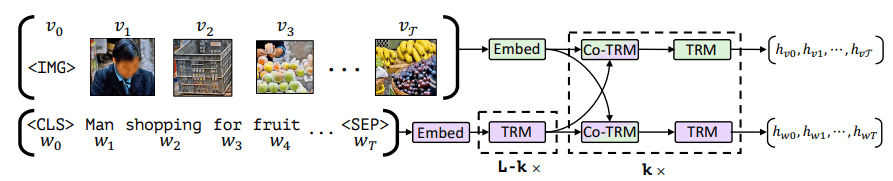
\includegraphics[width=1\textwidth]{figs/dual_stream_arc.png}}
        \caption{نمونه‌ای از یک مدل دوجریان}
        \label{fig:dual_stream}
    \end{figure}
}


\section{جمع‌بندی}
\paragraph{}
{
    در این فصل به شرح مفاهیم پایه‌ای پرداخته شد که در مراحل مختلف انجام
    این پژوهش مورد استفاده قرار گرفته و برای درک کامل خواننده‌ی
    این نوشتار مورد نیاز است.
    دراین فصل معماری‌ها و مدل‌های استفاده شده در این پزوهش به صورت جزیی مورد بررسی قرار
    گرفت. سپس به معرفی انواع مدل‌های موجود برای حل مسائل تصویر و زبانی پرداخته‌شد. 
}
